\documentclass[11pt]{scrartcl}
\usepackage{polski}
\usepackage[polish]{babel}

\usepackage{graphicx, float, caption, subcaption}
\usepackage{amsmath}
\usepackage{tabularx}
\usepackage{multirow}
\graphicspath{{images/}}

\title{Laboratorium 2 - Otoczka wypukła}
\author{Mateusz Podmokły}
\date{18 październik 2023}

\begin{document}
    \maketitle
    \section{Specyfikacja użytego środowiska}
    Specyfikacja:

    \begin{itemize}
        \item Środowisko: Jupyter Notebook,
        \item Język programowania: Python,
        \item System operacyjny: Microsoft Windows 11,
        \item Architektura systemu: x64.
    \end{itemize}
    \section{Przebieg ćwiczenia}

    Ćwiczenie polega na zaimplementowaniu algorytmów Grahama i Jarvisa obliczających
    otoczkę wypukłą oraz na analizie ich wyników.

    \subsection{Losowanie punktów}

    Wylosowane zostały następujące zbiory punktów:

    \begin{enumerate}
        \item losowo wygenerowane punkty o współrzędnych z przedziału
        \([-100,100]\),
        \item losowo wygenerowane punkty leżące na okręgu o środku
        \((0,0)\) i promieniu $R=100$,
        \item losowo wygenerowane punkty leżące na bokach prostokąta
        o wierzchołkach
        
        $(-10, 10)$, $(-10,-10)$, $(10,-10)$, $(10,10)$,
        \item punkty na wierzchołkach kwadratu $(0, 0)$, $(10, 0)$, $(10, 10)$,
        $(0, 10)$ oraz punkty wygenerowane losowo na dwóch bokach kwadratu
        leżących na osiach i na przekątnych kwadratu.
    \end{enumerate}

    \begin{figure}[H]
        \centering
        \begin{minipage}{0.45\linewidth}
          \centering
          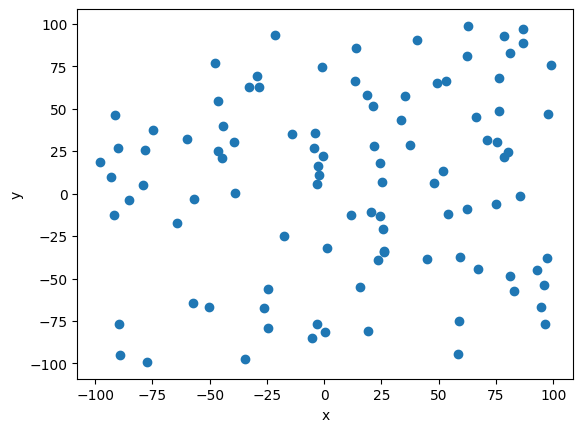
\includegraphics[width=1\linewidth]{2_1.png}
          \caption{Zbiór 1. - obszar kwadratowy.}
        \end{minipage}
        \begin{minipage}{0.45\linewidth}
          \centering
          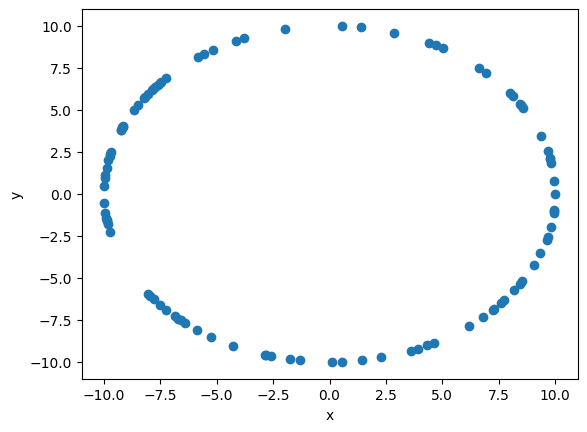
\includegraphics[width=1\linewidth]{2_2.png}
          \caption{Zbiór 2. - okrąg.}
        \end{minipage}
    \end{figure}

    \begin{figure}[H]
        \centering
        \begin{minipage}{0.45\linewidth}
          \centering
          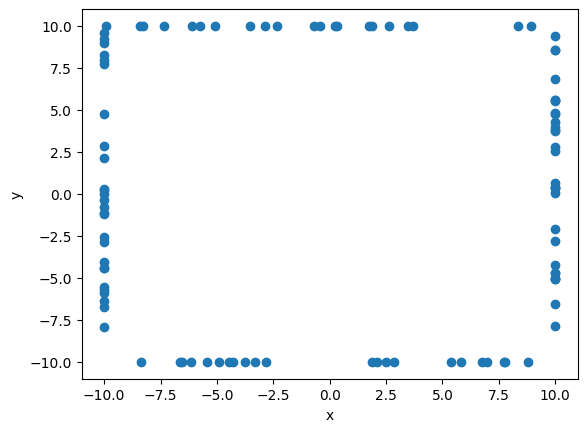
\includegraphics[width=1\linewidth]{2_3.png}
          \caption{Zbiór 3. - boki prostokąta.}
        \end{minipage}
        \begin{minipage}{0.45\linewidth}
          \centering
          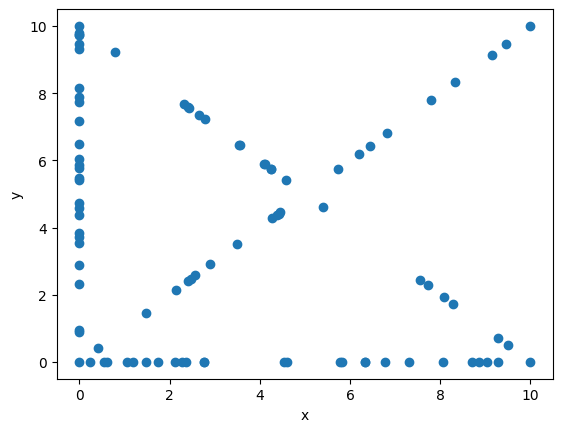
\includegraphics[width=1\linewidth]{2_4.png}
          \caption{Zbiór 4. - wierzchołki, boki i przekątne kwadratu.}
        \end{minipage}
    \end{figure}

    \subsection{Znajdowanie otoczki wypukłej}
    \subsubsection{Wykorzystane algorytmy i rodzaje pomiarów}
    Dla każdego zbioru obliczona została otoczka wypukła z użyciem algorytmu
    Grahama oraz algorytmu Jarvisa dla trzech różnych liczbach punktów
    w celu zwiększenia wiarygodności pomiarów. Zmierzony został czas każdego
    wykonania algorytmu.

    \subsubsection*{}
    Złożoności obliczeniowe algorytmów:
    \begin{itemize}
        \item Algorytm Grahama - $O(nlogn)$
        \item Algorytm Jarvisa - $O(kn)$, $k$ - liczba punktów otoczki
    \end{itemize}

    \subsubsection{Otoczki wypukłe przykładowych zbiorów}
    \begin{figure}[H]
        \centering
        \begin{minipage}{0.45\linewidth}
          \centering
          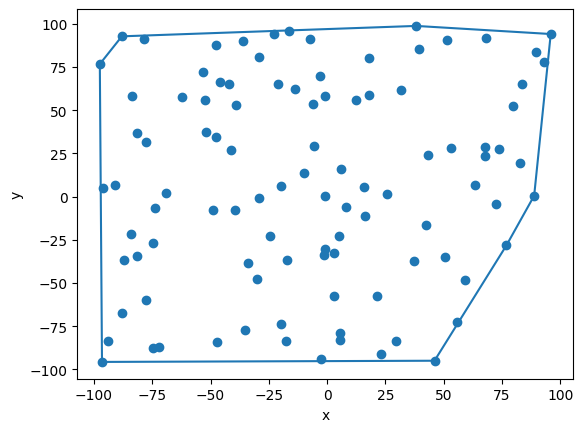
\includegraphics[width=1\linewidth]{2_5.png}
          \caption{Zbiór 1.}
        \end{minipage}
        \begin{minipage}{0.45\linewidth}
          \centering
          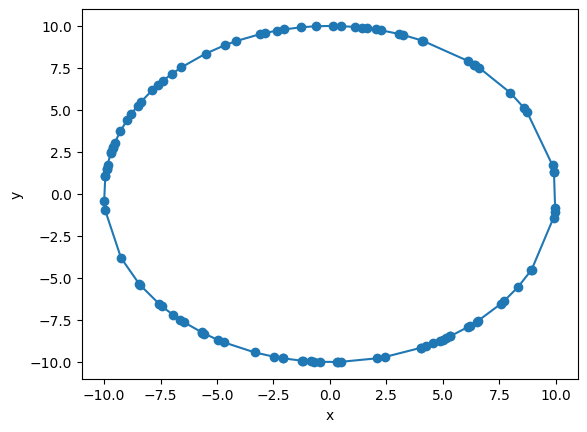
\includegraphics[width=1\linewidth]{2_6.png}
          \caption{Zbiór 2.}
        \end{minipage}
    \end{figure}

    \begin{figure}[H]
        \centering
        \begin{minipage}{0.45\linewidth}
          \centering
          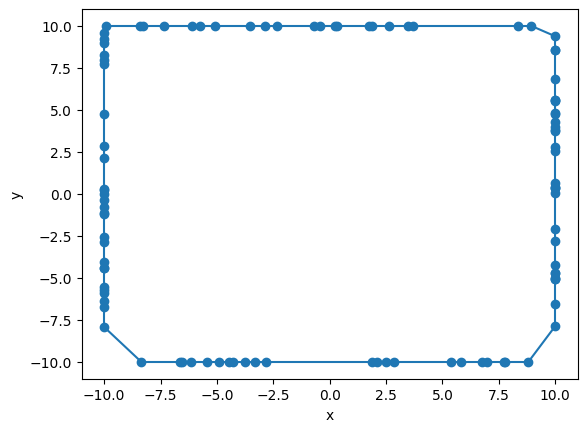
\includegraphics[width=1\linewidth]{2_7.png}
          \caption{Zbiór 3.}
        \end{minipage}
        \begin{minipage}{0.45\linewidth}
          \centering
          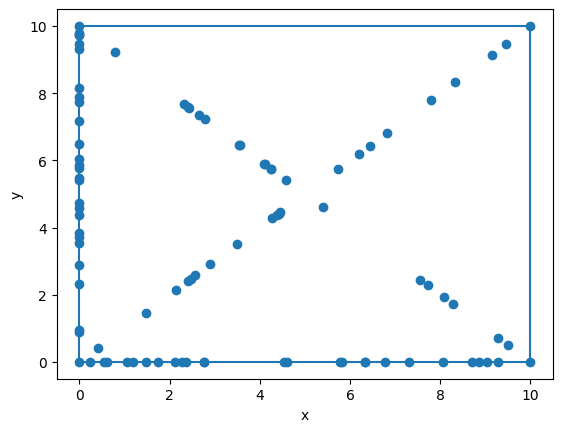
\includegraphics[width=1\linewidth]{2_8.png}
          \caption{Zbiór 4.}
        \end{minipage}
    \end{figure}

    \subsubsection{Liczności zbiorów użytych w poszczególnych pomiarach}
    \begin{enumerate}
        \item[-] Zbiór 1. - 10 000 punktów, 100 000 punktów, 1 000 000 puntków,
        \item[-] Zbiór 2. - 1000 punktów, 5000 punktów, 10 000 punktów,
        \item[-] Zbiór 3. - 10 000 punktów, 100 000 punktów, 1 000 000 puntków,
        \item[-] Zbiór 4. - 10 000 punktów, 100 000 punktów, 1 000 000 puntków.
    \end{enumerate}

    \section{Analiza wyników}
    \subsection{Zestawienie czasów działania algorytmów}

    \begin{table}[H]
        \centering
        \renewcommand{\arraystretch}{2}
        \begin{tabular}{| c | c | c | c | c |}
            \hline

            \multicolumn{2}{| c |}{\multirow{2}{*}{}} &
            \multicolumn{3}{c |}{Czas działania algorytmu} \\
            \cline{3-5}
            \multicolumn{2}{| c |}{} & Pomiar I & Pomiar II & Pomiar III\\
            \hline
            \multirow{2}{*}{Zbiór 1.} & Algorytm Grahama & 0.07 s &
            0.74 s & 11.02 s \\
            \cline{2-5}
             & Algorytm Jarvisa & 0.09 s & 1.06 s & 12.86 s \\
            \hline
            \multirow{2}{*}{Zbiór 2.} & Algorytm Grahama & 0.01 s &
            0.04 s & 0.09 s \\
            \cline{2-5}
             & Algorytm Jarvisa & 0.53 s & 15.01 s & 59.03 s \\
            \hline
            \multirow{2}{*}{Zbiór 3.} & Algorytm Grahama & 0.09 s &
            1.15 s & 14.45 s \\
            \cline{2-5}
             & Algorytm Jarvisa & 0.05 s & 0.44 s & 4.33 s \\
            \hline
            \multirow{2}{*}{Zbiór 4.} & Algorytm Grahama & 0.64 s &
            3.56 s & 41.3 s \\
            \cline{2-5}
             & Algorytm Jarvisa & 0.11 s & 0.42 s & 3.59 s \\
            \hline
            \end{tabular}
        \renewcommand{\arraystretch}{2}
        \caption{Czasy działania dla poszczególnych zbiorów i algorytmów.}
    \end{table}

    \subsection{Analiza otrzymanych czasów}
    Z Tabeli 1. wynika, że Algorytm Jarvisa osiąga lepszy czas niż Algorytm
    Grahama w przypadku zbioru 3. i 4. (odpowiednio punkty na bokach prostokąta
    i na bokach oraz przekątnych kwadratu). Natomiast w zbiorze 1. i 2.
    (odpowiednio losowa chmura punktów i okrąg) przewagę uzyskuje Algorytm
    Grahama, szczególnie dla zbioru, w którym punkty zlokalizowane są na okręgu
    różnica jest znacząca.

    \section{Wnioski}
    \subsection*{Szybkość porównywanych algorytmów}
    Czas działania Algorytmu Jarvisa jest zależny od liczby punktów należących
    do otoczki, natomiast Algorytm Grahama zawsze działa w czasie $O(nlogn)$.
    Otoczka wypukła zbioru 3. może składać się z maksymalnie ośmiu punktów (po
    dwa na każdy bok prostokąta), a zbioru 4. zawsze z dokładnie czterech (jeden
    w każdym rogu kwadratu), dlatego czas wykonania Algorytmu Jarvisa będzie tutaj
    znacznie krótszy. Zbiór, w którym wszystkie punkty położone są na okręgu (2.)
    charakteryzuje to, że każdy punkt wchodzi w skład otoczki. Wtedy złożoność
    rośnie do $O(n^2)$, więc o wiele szybszy będzie Algorytm Grahama. Zbiór 1.
    to losowa chmura punktów rozmieszczonych wewnątrz prostokąta. Czas obydwu
    algorytmów jest tutaj zbliżony, z lekką przewagą Algorytmu Grahama ze
    względu na to, że liczba punktów otoczki takiej chmury punktów jest zazwyczaj
    większa od $log_2n$, gdzie $n$ to liczba wszystkich punktów.

    \subsection*{Podsumowanie}
    Algorytm Grahama lepiej sprawdza się w przypadku, gdy znaczna część puntków
    należy to otoczki wypukłej zbioru ze względu na to, że jego złożoność nie
    zależy od ich liczby. Z kolei Algorytm Jarvisa warto użyć jeżeli wiemy, że
    otoczka składa się z niewielkiej liczby punktów, dokładnie jeżeli
    $k < log_2n$.

\end{document}
